Since the beginning of the 2000s, knitting has encountered a steady rise in popularity (\cite{lewis_rise_of_knitting}). This, Lewis says, might be due to the rise of the internet and social media, and the increasingly important role they play in the daily life. The older knitting generation is adapting to new technology and switching over, Lewis explains, bringing knitting as a craft and hobby closer to the younger generations (\cite{lewis_rise_of_knitting}). Online communities like Ravelry\footnote{\url{http://www.ravelry.com/}} and Youtube\footnote{\url{https://www.youtube.com/}} teach the knitting enthusiasts knittings techniques and patterns of all kinds --- never has knitting knowledge been more accessible.

Considering this, it is all the more surprising that there are only few apps related to knitting to be found on the Play Store, Google's digital distribution service for Android apps. Only one app supports the creation of a knitting pattern chart. Mobile devices have the potential to be a great help to knitters. An app could help knitters keep track of the projects they are currently knitting, look up instructions, and store knitting patterns. The latter especially aids the mobile knitter --- no longer is it necessary to carry sheets of paper with pattern charts or even books, as seen in \reffigure{fig:knitting_book}, around.

\begin{figure}[H]
	\centering
    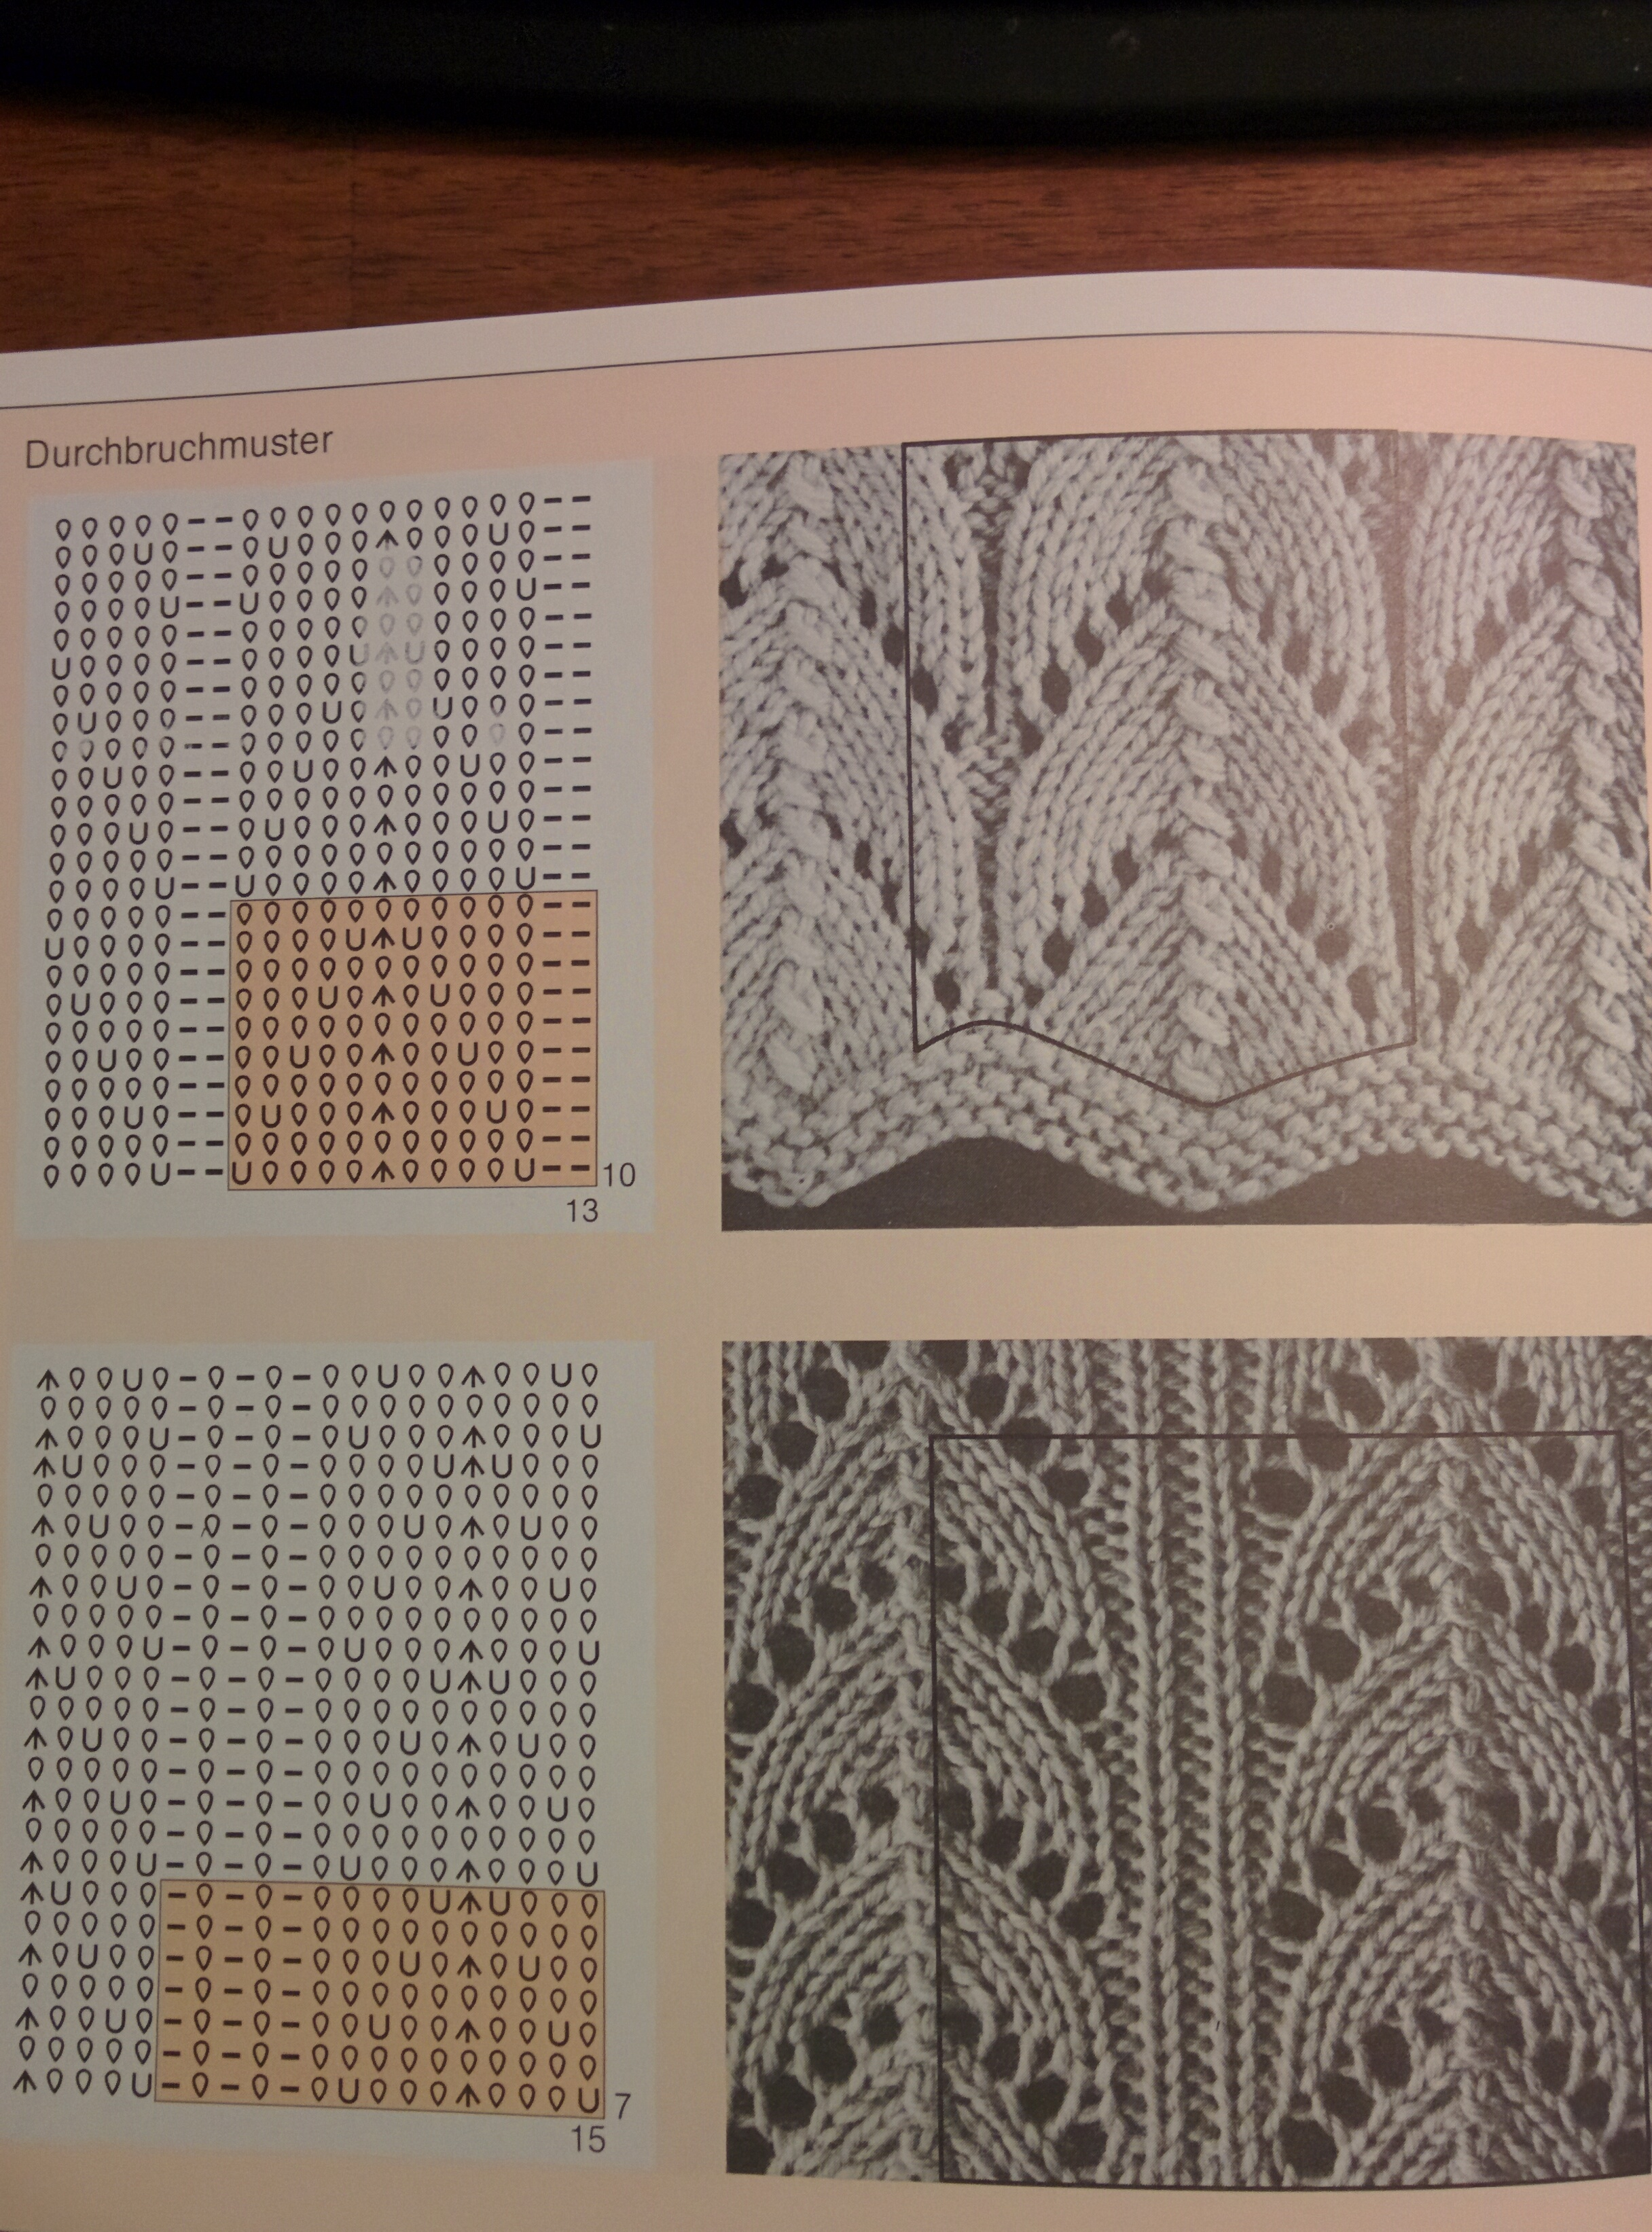
\includegraphics[width=.45\textwidth]{images/knitting_pattern_chart_book.jpg}
   \caption[{Knitting patterns and their corresponding pattern charts \protect\newline{\small from \protect\cite[p142]{Natter1983}}}]{Knitting patterns and their corresponding pattern charts from \protect\cite[p142]{Natter1983}}
   \label{fig:knitting_book}
\end{figure}

Displaying a pattern chart on a mobile device is difficult because of the small size of the screens of contemporary mobile devices. This screen is a far smaller medium than a sheet of paper, on which pattern charts are normally printed. 

Pattern charts, excluding the smaller charts, are therefore too big to be viewed easily inside an app. The goal for this thesis is to research how a knitting pattern chart can be input and displayed on mobile devices running the Android operating system and develop a working prototype showcasing the results of that research. The prototype will be evaluated through testing by users representative of the prototype's target group. This testing will, if time permits, be executed iteratively throughout developement to ensure a useful \gls{UI} design. The term useful in this context is taken from the article \textit{Usability 101: Introduction to Usability} by \cite{nielsen2014} --- he uses the term to summarize the usability and utility of a design. Nielsen furthermore defines utililty and usability as indicators of ``[...] whether [a design] provides the features you need'' and ``how easy [and] pleasant these features are to use'' (\cite{nielsen2014}).